\section{Camera Module}
\label{sec:John_Implementation}

The first step in the implementation of the camera module was to verify the communication with the camera by talking to it via a pc. Once this step was complete the next step was to implement communications between the camera and a microprocessor, with the pc for debugging. With the microcontroller able to communicate with the camera this module was ready for integration with the payload.

\subsection{First camera}

The first attempt at communicating with the original camera was done using the arduino microcontroller board. The arduino was chosen as the platform for this first communication because it is simple to program and its programming environment provides various useful libraries, for example for serial communication. The hardware also provides an easily accessible serial port.

The first implementation of this code managed to occasionally sync with the camera but would generate errors after this point. After examining the code and the camera's datasheet it was discovered that the camera was only syncing occasionally because the arduino was using a slower baud rate than the camera could auto-detect, after increasing the baud rate on the arduino the camera would sync every time but the code still generated errors after this point.

It was at this point that the first camera broke. It was no longer syncing at all where before it had been doing so reliably and so it was checked with one of the bench-top power supplies and was seen to be no longer drawing current properly.

\subsection{Second camera}

Once it was established that the first camera was dead a couple of cheaper surface mount camera modules were purchased as possible replacements however making a successful connection to these components proved excessively difficult so a new camera of the same type as the previous one was ordered.

\subsubsection{Serial cable to computer}

The operation of the new camera module was verified using a usb to serial cable connected to a pc which was running the sample program which was provided by the camera's manufacturer. Using this set up it was shown that the camera was working and that it was possible to get images from it.

[] diagram of pin connections []

\subsection{Arduino implementation}

With the operation of the camera verified it was reconnected to the arduino board and the code run again with the same result as before: it would correctly sync but no more than this. On inspection of the code it became clear that this was because the same serial line was being used for both communication with the camera and debug messages and that these debug messages were interfering with further communications. Debug messages were therefore moved to a software serial line and sent to the computer via the usb to serial cable and observed using PuTTy.

The code is broken down so that there are functions for each type of command that the camera can receive, functions that verify the responses from the camera and functions that combine these together in the correct sequence in order to perform a useful task with the camera.

\subsubsection{Camera synchronisation}

The first task in communicating with the camera is to synchronise the serial channel, the uCam datasheet gives the correct protocol to do this.

\begin{figure}[H]
        \centering
        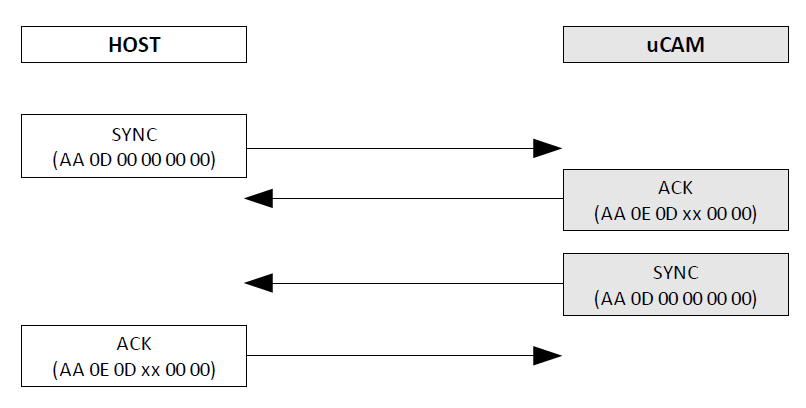
\includegraphics[width=1.00\textwidth]{figures/SyncProtocal.png}
        \captionof{figure}{Command protocol for synchronisation, sourced from \cite{ucam_datasheet} }
        \label{fig:syncProto}
\end{figure}

It should be noted that in \ref{fig:syncProto} the first sync sent from the host will be repeated until an acknowledgement is received, with everything working correctly this process usually takes 3 or 4 syncs before an ACK is received.

The inclusion of a separate debugging line allows for messages at each stage of this process to verify that it is connecting correctly and to indicate where any errors may have occurred. With all debug messages enabled this function will output "Sending syncs" followed by a "." for each sync command sent and then "ACK received" and "SYNC received", the main code will then output a message to the effect that contact has been successfully established.

\subsubsection{Taking a snapshot}

With the camera successfully synchronised the controller needs to be able to trigger the camera to take a photograph and then retrieve said photograph, again the uCam datasheet gives an example of how to implement this.

\begin{figure}[H]
        \centering
        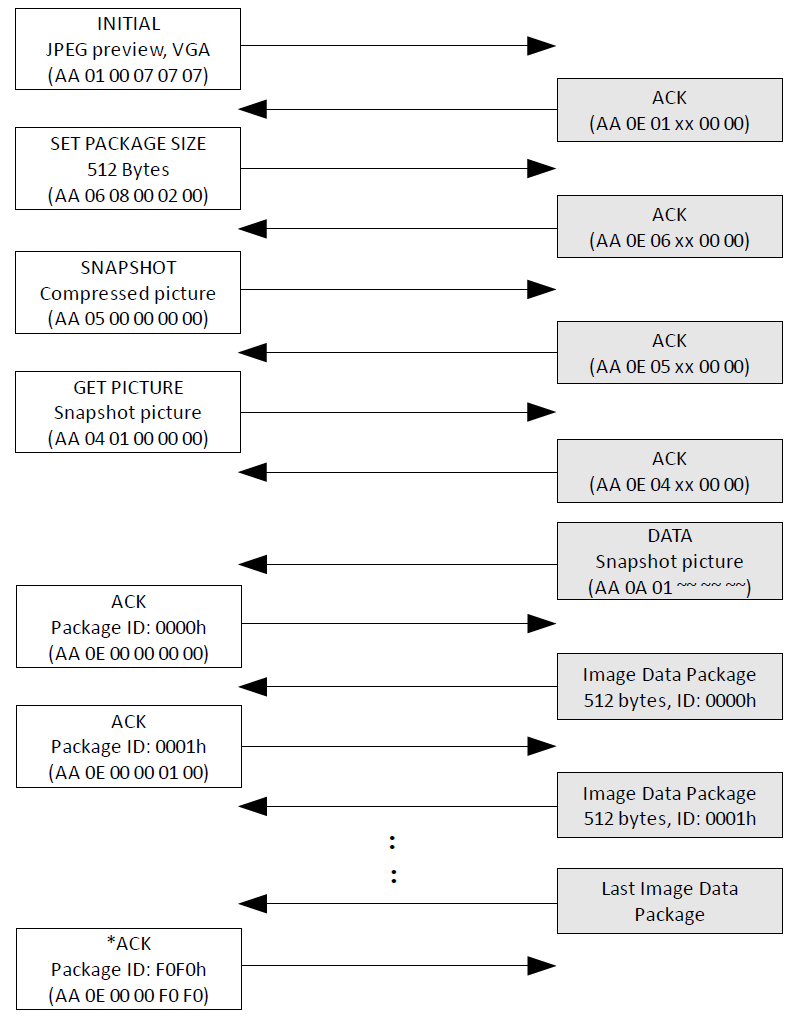
\includegraphics[width=1.00\textwidth]{figures/SnapshotProtocal.png}
        \captionof{figure}{Command protocol for taking and retrieving a jpeg snapshot at 640x480 resolution, sourced from \cite{ucam_datasheet} }
        \label{fig:snapProto}
\end{figure}

It should be noted in \ref{fig:snapProto} that the values in the commands are for the example and are not necessarily the values used in the code.

The "INITIAL" command has parameters that allow the image type and resolution to be set, in \ref{fig:snapProto} the image type is set to jpeg and the resolution is set to 640x480, these values are kept as the standard in the code.

The "SET PACKAGE SIZE" command is only relevant for jpeg images and set the size of the data packages that are sent when one requests an image. In \ref{fig:snapProto} this value is set to 512 bytes however in the code this is set to 64 bytes as it was originally thought that the system might have to transmit these packages as soon as receiving them so they needed to be a reasonable size to fit in with the timing between transmit packets sent by the autopilot.

The "SNAPSHOT" command tells the camera to take a single picture, its parameter sets whether the image is jpeg compressed or raw, in \ref{fig:snapProto} this is set to be a jpeg image and this is left as the default in the code.

The last command sent by the controller is the "GET PICTURE" command which tells the camera to send image data, it has one parameter which sets which image is sent. In \ref{fig:snapProto} this is set to send the snapshot image and this is also how it is set in the code. As well as sending back an ACK this function will also send back a "DATA" message which tells the controller what type of image is being returned and how large it is.

Once the controller has acknowledged the "DATA" message the camera starts to send data packages, each of which needs to be acknowledged, until the entire image is transferred. Whilst this process is going on the data packages are saved to an SD-card as described in [] ref to andy's section [].

The use of the debug communication channel again allowed for detailed analysis of this process with the maximum amount of debug messages being one before each command is sent saying what that command is and another message once and ACK is received, there is also then a message with the size of the data in and then messages with the package number and the byte number within that package, the data can also be output to the debug channel.

[] screenshots of debug channel, with camera disconnected and with it connected []

\subsection{Miscellaneous Problems}

Before the SD-card was implemented the sending of the data directly via the debug channel was attempted and so was its reconstruction into a jpeg image on the computer, this could not be made to work however. On looking at the data as it came off the arduino via the software serial debug line it became clear (particularly when looking at the counting values, whose values were already known) that the data was not being transmitted reliably. For this reason this method of getting an image was abandoned, this also had to taken into consideration whilst thinking about the integration of this part of the system as the software serial line is not a reliable method of transmitting the data some other method would have to be used.

Another problem that was noticed after the camera control had been integrated, as described in [] ref to mike's section [], was that every other time the system was powered up the camera would require a reset/power cycle. This was discovered to be because the Rx wire to the camera was left floating, this was fixed by the addition of a 10k$\Omega$ pull-up resistor.

It was also noticed quite early on that the camera required 3.3V logic levels but the arduino outputs 5V logic levels, the arduino could receive logic at 3.3V easily enough but the 5V output was causing occasional errors. In order to fix this problem the 5V output from the arduino was taken through a potential divider of a 10k$\Omega$ resistor and a 3V zener diode.